\chapter{Regularisation of Models}
\label{ch:regularisation-of-models}\index{regularisation-of-models|(}


\section{Introduction}


\textit{Regularisation of Models} deals with the widespread problem of overfitting in machine learning (ML) models. In a supervised learning setting with many input features, overfitting is usually a potential problem unless there is ample training data \citep{ng2004feature}. When a machine learning model is overfitting it implies that the model has been trained in such a way to perform well on the particular training data but perform badly when using test or unseen data. The over-fitting model learns the pattern as well as the noise in the training data. This occurs when the model has a high variance and when there is a highly complex model with respect to the underlying data \citep{pythonmachinelearning}. The other extremity is under fitting where the model has a high bias. High variance refers to the variability of the model output prediction for different test inputs, whereas bias refers to the errors due to the `assumptions` of the model that differ from the actual. Therefore, the challenge is to find a good bias-variance trade-off. This concept is illustrated in Figure~\ref{fig:rom_overfitting}.


\begin{figure}
   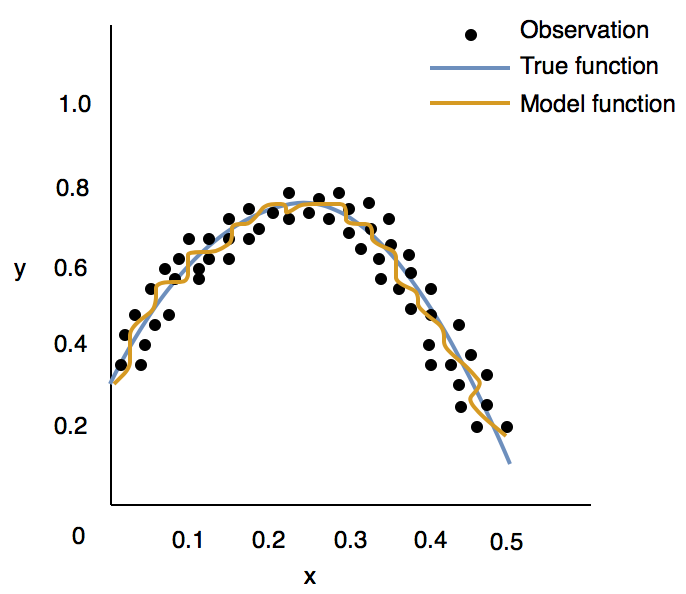
\includegraphics{regularisation_of_models/overfitting.png}
  \caption{Overfitting and Underfitting: Challenge for a good bias-variance trade-off}
  \label{fig:rom_overfitting}
\end{figure}


The \textit{compromise} or \textit{generalisation} challenge can be tackled using regularisation techniques. A number of regularisation techniques will be discussed in this chapter. The techniques include i) L1 regularization, ii) L2 Regularization, iii) Dropout, and iv) Early Stopping. The next sections describes these regularisation techniques.


\section{L2 and L1 regularization} \index{L2 and L1 regularization}


Regularization is a technique which makes slight modifications to the learning algorithm such that the model generalises better. This generalisation is achieved by introducing a bias  so that the overfitted example in Figure~\ref{fig:rom_overfitting} can shift to the left. The learning algorithms such as regression and deep learning typically learn using a cost or error function which is minimized such that the model with minimum error is determined.

Figure~\ref{fig:rom_traineval} illustrates a typical plot of the error function versus the number of iterations for the `Training Data` and `Validation Data`. At each iteration the validation data is used to test out the model being trained. As can be noticed although the error function typically is minimized and converges, the `Validation Data` does not. This is due to the overfitting problem introduced earlier. 

\begin{figure}
   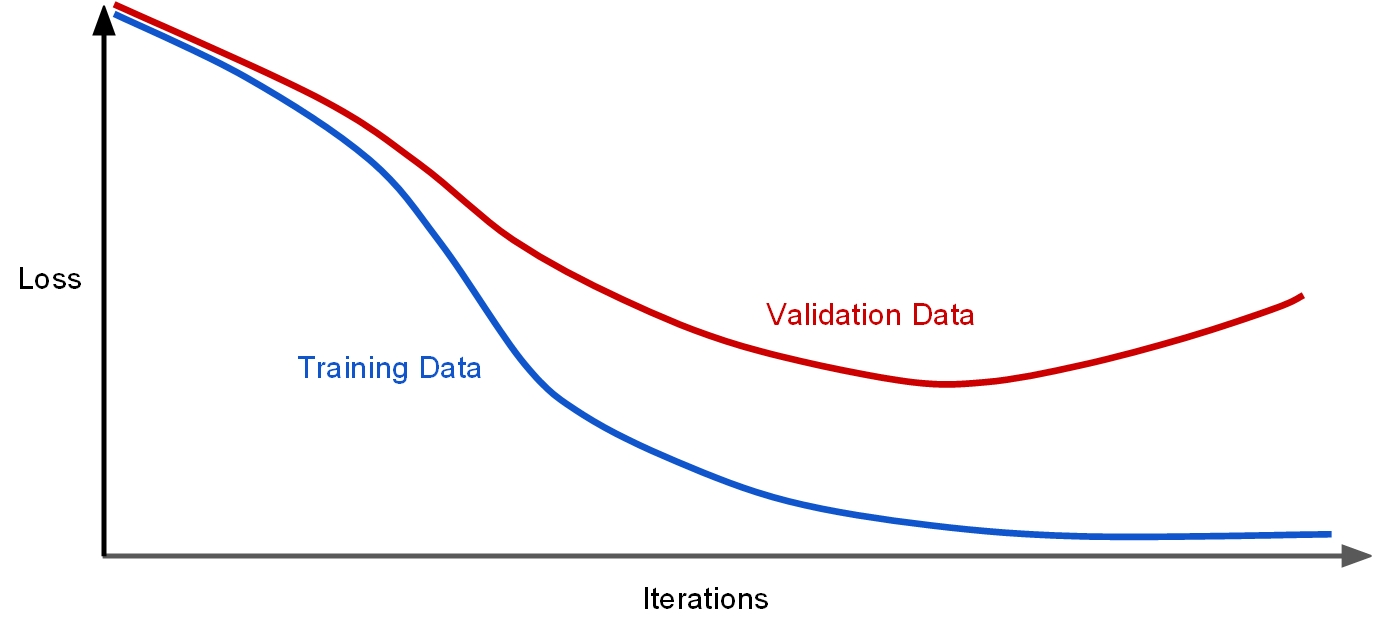
\includegraphics{regularisation_of_models/trainingVseval.png}
  \caption{Training Data Error, and Validation Data Error Vs Iterations}
  \label{fig:rom_traineval}
\end{figure}


Regularisation uses a \textit{regularisation} parameter $\lambda$ to add the bias or penalty to the error function as the model complexity increases. Function \ref{eq:rom_penalty}  defines a simplified loss/cost function with regularisation.

\begin{equation}
\label{eq:rom_penalty}
minimize ( cost function, c(x) + \lambda(penalty function) )
\end{equation}

Function  \ref{eq:rom_penalty} includes two terms; i) the cost function, and ii) the penalty (regularization) function, where the penalty function is constrained to be less than or equal to a constant, t \citep{friedman2001elements}.

To train the model, minimisation is done on both the cost and penalty functions. The cost function, c(x) depends on the training data whereas the regularisation function is independent of the data variable ($x_n$). Parameter $\lambda$ is determined empirically or through cross validation, and it is used to control how to balance out the two terms in function \ref{eq:rom_penalty}  $-$ balance how much the model should learn the training set, and how much bias to add to the model. There are two methods for regularisation that apply a bias which are termed L2 and L1, known as Ridge and Lasso Regression respectively. L2 and L1 penalize weights differently.




\subsection{L2 Regularisation} \index{L2 and L1 regularization!L2 Regularisation}


L2 regularisation penalizes the $weight^2$. Therefore, considering the cost function for linear regression as an example, function \ref{eq:rom_penalty} can be re-written as:

\begin{equation}\label{rom_l2}
minimize ( \sum^{n}_{i=1}(y_i - w_0 - \sum^{p}_{j=1}(x_ij.w_j) )^2 + \lambda\sum^{p}_{j=1}(w_j^2) )
\end{equation}

Where $y_i$ is the predicted value from which the actual value is subtracted. The weight, ($w_0$) (intercept in linear regression) is left of out the penalty function. In L2 regularisation $\lambda$ is a complexity parameter that controls the amount of shrinkage \citep{friedman2001elements}.  The idea of penalizing by the $weight^2$ is also used in neural networks where it is known as weight decay \citep{krogh1992simple,moody1992effective}. \citet{krogh1992simple}, claim that the ``generalisation ability of a Neural Networks depend on a balance between the information in the training example and the complexity of the network``, where the complexity is related to the number of weights in the model. L2 regularisation tries to minimize the number of weights, and therefore make the model less complex, whilst still minimizing the error. Anders and John have shown that weight decay improves generalisation by i) suppressing the irrelevant weights, and ii) suppressing the effect of static noise. 



\subsection{L1 Regularisation} \index{L2 and L1 regularization!L1 Regularisation}


On the other hand, L1 penalizes on the |weight| \citep{friedman2001elements}. Therefore the function is rewritten as:

\begin{equation}\label{rom_l1}
minimize ( \sum^{n}_{i=1}(y_i - w_0 - \sum^{p}_{j=1}(x_ij.w_j) )^2 + \lambda\sum^{p}_{j=1}(w_j) )
\end{equation}

The derivative of L2 and L1 regularisation term would result in 2w and k (a constant) respectively (considering penalty function only), when computing partial derivatives with respect to the weights, ($w_n$). Therefore, L2 regularisation removes a percentage from the weight, whereas L1 subtracts a constant from the weight. This creates a significant difference from the Ridge function as it will cause some of the coefficients to be exactly zero for an appropriate value of t \citep{friedman2001elements}. L2 regularization encourages weights to be small, but doesn't force them to exactly zero.

\citet{ng2004feature} considered supervised learning problems where the feature space is made up of many irrelevant features (noisy), and studied L1 and L2 regularization applied on logistic regression methods for preventing over-fitting. L1 regularisation cause the weights of some features to go to zero, making it highly suitable for models where many of the features should be ignored. He has found L1 regularisation to be effective in these scenarios and concluded that L1 regularized logistic regression can be effective even if there are exponentially many irrelevant features as there are training examples.


Since L1 regularisation encourages the weight for meaningless features to drop to exactly 0, consequently being removed from the model, it makes this technique suitable for sparse datasets where there could be potentially considerable meaningless features or dimensions. On the other hand L1 regularisation can have the negative affect that it zeros the weight for weakly informative dimensions. 


\section{Dropout} \index{Dropout}

Dropout is another regularisation technique that is targeted for neural networks (NN) models. Overfitting is a serious problem in deep neural nets and\citet{srivastava2014dropout} have proposed the dropout technique to tackle this challenge. \citet{wager2013dropout} has described dropout as a method that ``falls into the broader category of learning methods that artificially corrupt training data to stabilize prediction``.

The key idea as described by Srivastava is to ``drop units (along with their connections) from the neural network during training`` at each iteration. This dropout regularizing method can also be interpreted as a way to add noise to the hidden layers of the NN, similar to the regularising functions described in the previous section for L1 and L2. The dropout technique is illustrated in Figure~\ref{fig:rom_dropout_a},\ref{fig:rom_dropout_b}. 

\begin{marginfigure}%
	\centering
	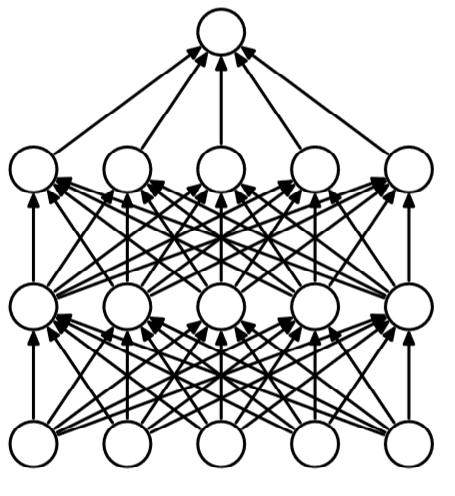
\includegraphics[width=\linewidth]{regularisation_of_models/dropout_a.png}
	\caption{Standard Neural Net}
	\label{fig:rom_dropout_a}
\end{marginfigure}
\begin{marginfigure}%
	\centering	
	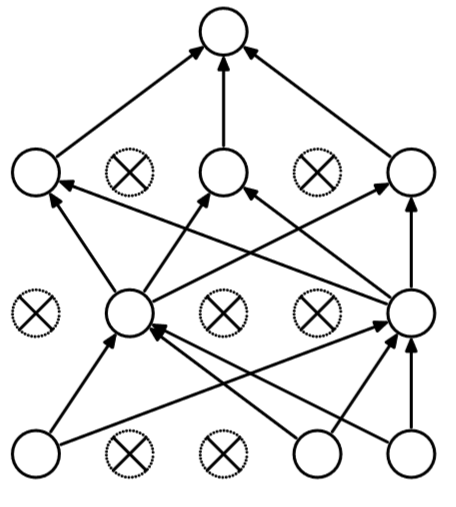
\includegraphics[width=\linewidth]{regularisation_of_models/dropout_b.png}
	\caption{Thinned Neural Net after applying dropout}
	\label{fig:rom_dropout_b}
\end{marginfigure}


The dropout is a random action and is only used during the train phase. Therefore at each iteration a different thinned NN Figure~\ref{fig:rom_dropout_b} is used for training. The intensity of the dropout is regulated by another hyperparameter $p$, describing the probability of retaining a unit, where $p=1$ implies no dropout. Dropout can be applied both for the input layer and also for hidden layers. \citet{srivastava2014dropout} have determined that the typical values of $p$ for hidden layers is between 0.5$-$0.8, whilst for real-valued inputs 0.8 is used. An incorrect value of $p$ may lead to underfitting.

For the testing phase all neurons use an averaging technique to combine weights from the different \textit{thinned} NN (Figure~\ref{fig:rom_dropout_b}) that were used during training. If a NN unit was retained with probability $p$ during training, the outgoing weights for that unit are multiplied by $p$ at test time. The result is a single unthinned network that has smaller weights which is then used for testing.

This technique was found to improve the performance of NN across application domains including object classification, digit recognition, speech recognition, document classification, and analysis of computational biology data. Therefore, \citet{srivastava2014dropout} concluded that the dropout method is a general technique that can be applied across different domain. Dropout has a drawback that it extends the training time by typically 2$-$3 times \citep{srivastava2014dropout}. \citet{wager2013dropout} show that the dropout regularization is first-order equivalent to an L2 regularize applied after scaling the features by an estimate of the inverse diagonal Fisher information matrix, and have used this to improve the performance of dropout training. 



\section{Early Stopping} \index{Early Stopping}

Early stopping refers to a method where the training model is stopped before the training error is minimized (blue curve in Figure~\ref{fig:rom_traineval}), and is a method applied to NN \citep{Sarle95stoppedtraining}. The target is to stop the training before the validation error start increasing (red curve in Figure~\ref{fig:rom_traineval}). Richard M.Zur \citep{zur2009noise} et al showed that early stopping reduces the effect of overfitting but is it is not as effective as weight decay described earlier.





\index{Regularisation of Models|)}
